\begin{frame}\frametitle{Requirements for Selection of $W\gamma\rightarrow\mu\nu\gamma$ Candidates}
% ADD A PLOT WITH GEOMETRY (eta)
  \begin{table}[h]
     \tiny
     \begin{center}
     \begin{tabular}{|c|l|}
     \hline
      &  \\
     {\scriptsize{Selection requirements}} & {\scriptsize{Comment}} \\  
     &  \\ \hline

    {\scriptsize\bfseries\color{blue}{Event level selection criteria:}}  & \\ 
    Exactly one muon + at least one photon  & process signature\\  
     $M_T^W=>$40~GeV & process signature\\ 
     $\Delta{R}(\mu,\gamma)>$0.7 & theory consideration\\  \hline

     {\scriptsize\bfseries\color{blue}{Photon selection:}} & \\
     {\tiny{$P_T^{\gamma}>$15~GeV}} & theory considerations \\ 
     {\tiny{$\eta^{\gamma}$: ECal barrel (EB) or endcap (EE)}} & acceptance \\ 
     {\tiny{Photon ID}} & POG**-recommended \\ \hline

      {\scriptsize\bfseries\color{blue}{Muon selection:}} & \\
      \tiny{$p_T^{\mu}>$25~GeV;} & trigger\\ 
      \tiny{$|\eta^{\mu}|<2.1$} & trigger\\ 
      Muon ID & POG-recommended \\ \hline

      {\scriptsize\bfseries\color{blue}{Second muon veto:}} & rejects Z+jets, $Z\gamma$\\
      \tiny{$p_T^{\mu2}>10$ GeV;} &   \\
      \tiny{$|\eta^{\mu2}|<2.4$}  &     \\ \hline
      \end{tabular}
      \end{center}
  \end{table}
\scriptsize
If we have several candidates in an event, we choose one with the highest $P_T^{\gamma}$\\
\tiny
* ID - identification criteria\\
** POG - Particle Object Group (in CMS)\\
- - - - - - - -\\
$M_T^W=\sqrt{2  P_T^{l}  E_T^{miss}  (1-\cos{(\phi^{l}-\phi^{miss})})}$,  $\Delta{R}(\mu,\gamma)=\sqrt{ (\phi_\mu-\phi_\gamma)^2 + (\eta_\mu-\eta_\gamma)^2 }$
\end{frame}%{Event-Level Selection Requirements}

\begin{frame}\frametitle{$P_T^{\gamma}$ Spectrum of $W\gamma\rightarrow\mu\nu\gamma$ Candidates}
  \begin{figure}[htb]
    \begin{center}
       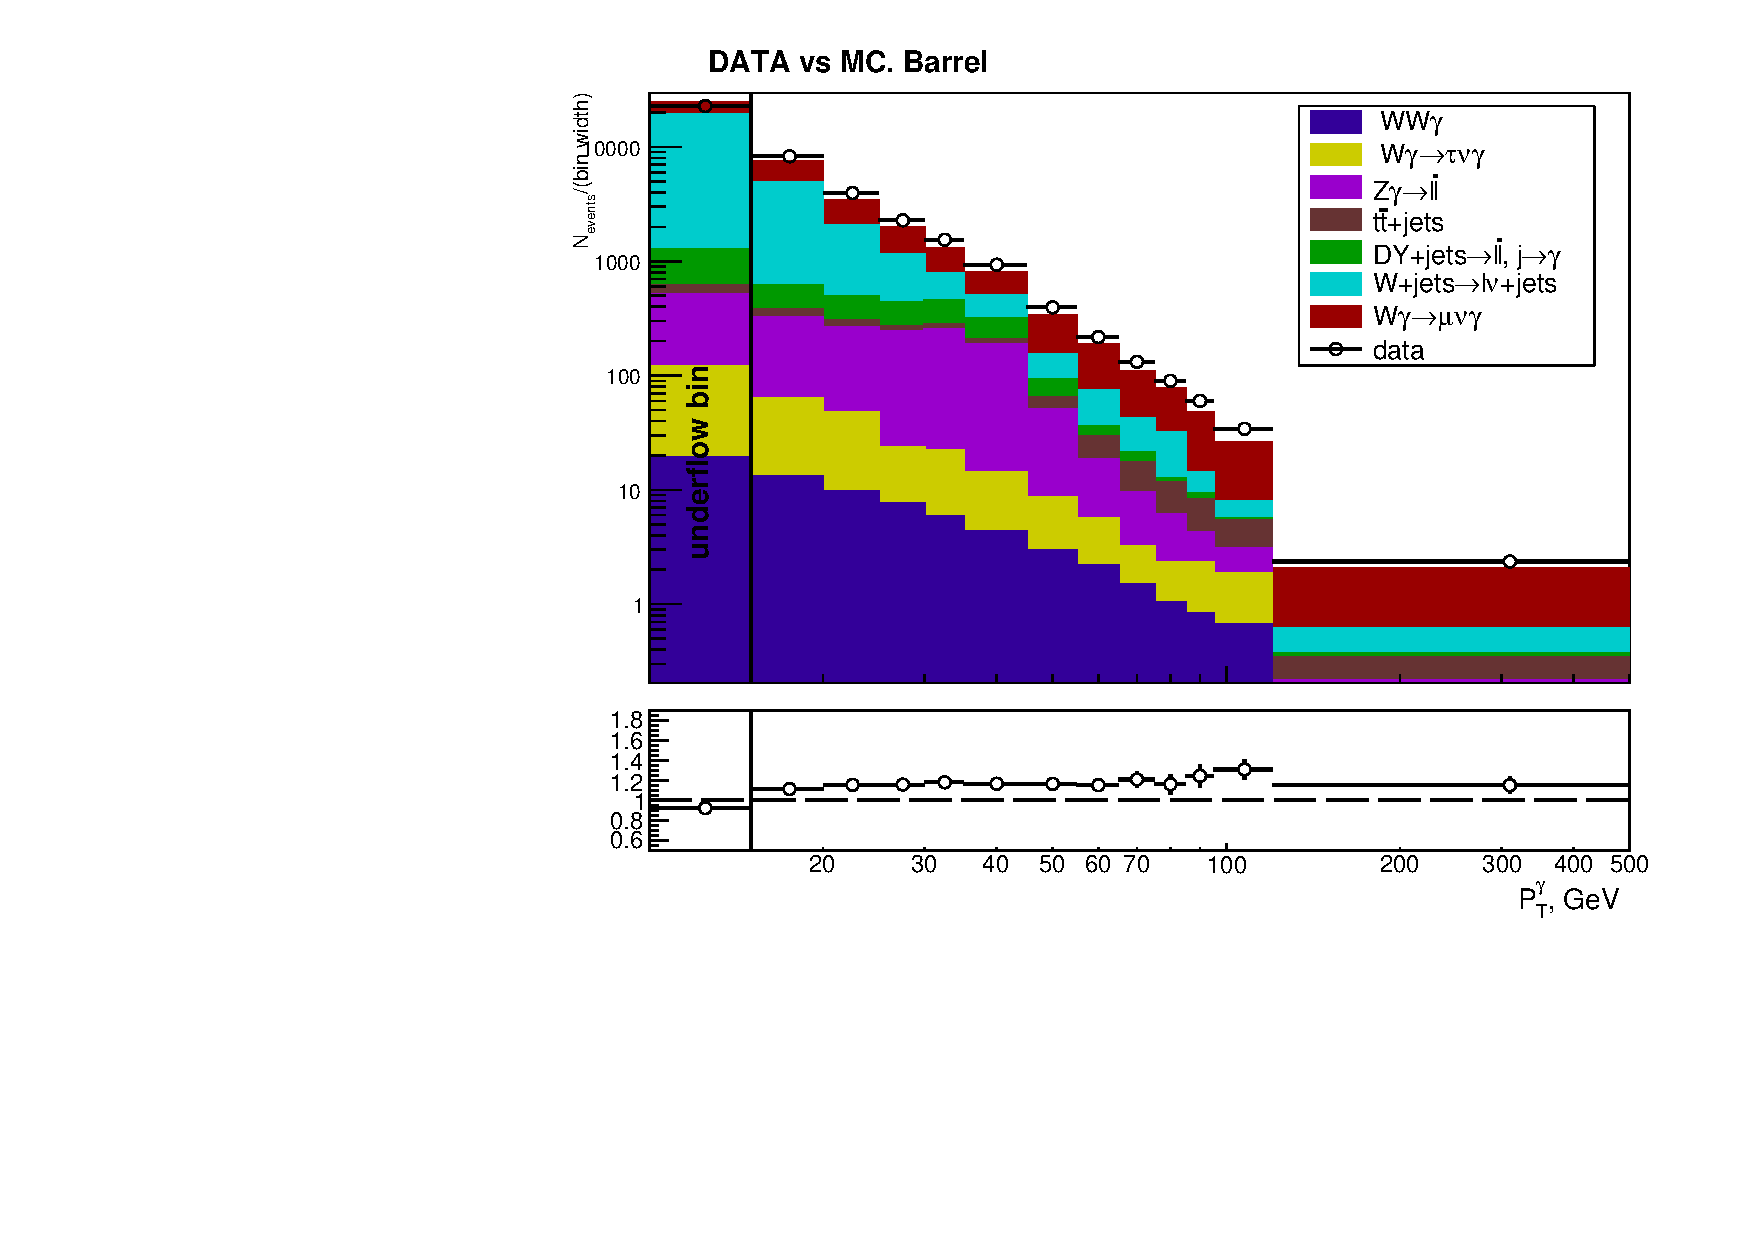
\includegraphics[width=0.65\textwidth]{../figs/figs_v11/MUON_WGamma/PrepareYields/c_TotalDATAvsMC_Barrel__phoEt.pdf}  
    \end{center}
  \end{figure}

\tiny
  \begin{table}[h]
     \tiny
     \begin{center}
     \begin{tabular}{|l|l|}
     \hline
     Dominated by $W$+jets* events in low $P_T^{\gamma}$ bins; &  {\bfseries{ Backgrounds:}}\\ 
     Fraction of signal increases with $P_T^{\gamma}$; & Jets$\rightarrow\gamma$: $W$+jets, DY+jets**, $t\bar{t}$+jets;\\
     Data disagree with MC. & Real-$\gamma$: $Z\gamma$, $W\gamma\rightarrow\tau\nu\gamma$.\\
     \hline
      \end{tabular}
      \end{center}
  \end{table}

* jets are hadronic jets (explained more later)\\
** DY+jets is Drell-Yan+jets process, can be understood as $Z$+jets

\end{frame}


